\documentclass[12pt]{article}
\usepackage[utf8]{inputenc}
\usepackage[spanish, mexico]{babel}
\usepackage[T1]{fontenc}
\usepackage{Alegreya}
\usepackage{euler}
\usepackage{graphicx}
\usepackage{hyperref}
\usepackage{geometry}

\geometry{
  top=10mm,
  bottom=10mm,
  left=10mm,
  right=10mm
}

\graphicspath{{./images/}}

\makeatletter
\def\@maketitle{
  \hbox{
    \noindent
    \fbox{
      \begin{minipage}{0.975\textwidth}
        \noindent
        \rlap{\makebox[25mm][l]{Alumno:}\@author}\hfill\llap{\textbf{\@title}}\\
        \rlap{\makebox[25mm][l]{No. Cuenta:}\texttt{\noCuenta}}\hfill\llap{\textit{\semestre}}\\
        \rlap{\makebox[25mm][l]{Correo:}\href{mailto:\correo}{\correo}}\hfill\llap{\textsc{\noTarea}}
      \end{minipage}
    }
  }\medskip
}
\makeatother

\title{Programación Declarativa}
\newcommand{\semestre}{2023\--1}
\newcommand{\noTarea}{Propuesta Proyecto}
\author{Erik Rangel Limón}
\newcommand{\noCuenta}{318159287}
\newcommand{\correo}{erikrangel.014@ciencias.unam.mx}

\begin{document}

\pagenumbering{gobble}

\maketitle

\section*{Cierre convexo para un conjunto de discos}

\noindent Este semestre estoy cursando la optativa de \textit{``Geometría Computacional''} para la cual voy a realizar una exposición sobre un artículo que explica un algoritmo para calcular un cierre convexo.

\medskip

El problema a resolver es el siguiente:

Se tiene un conjunto de $S$ discos en el plano de tamaño arbitrario que posiblemente se intersectan; se desea calcular el cierre convexo de $S$, es decir, la región convexa más pequeña que contiene a todos los discos en $S$.

La solución a este problema se realiza mediante un algoritmo con una estrategia ``divide y vencerás'' que divide el conjunto de discos y calcula recursivamente su cierre convexo, para posteriormente unir el cierre convexo con un algoritmo \textit{``merge''}.

\begin{figure}[h!]
  \centering
  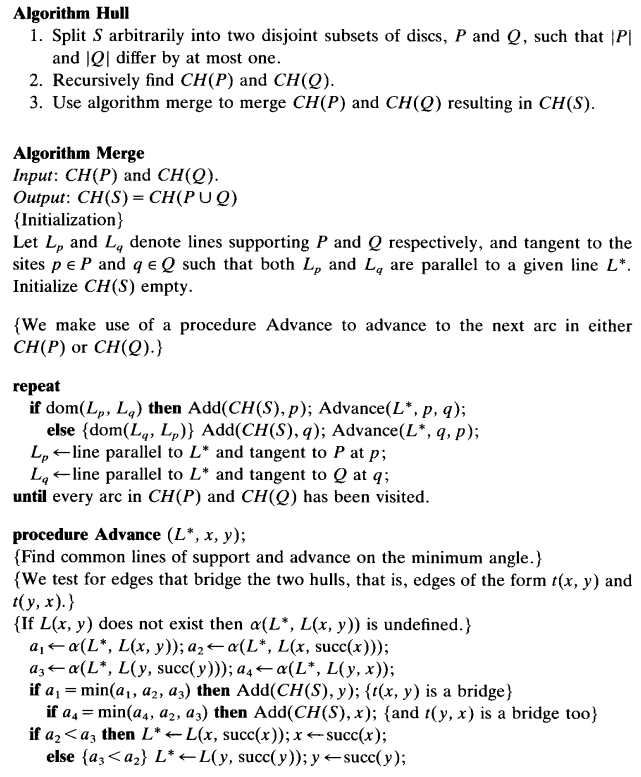
\includegraphics[width=0.7\textwidth]{hull.png}
  \caption{Algoritmo para calcular el cierre convexo}
\end{figure}

El algoritmo parece corto dado que utiliza algunas primitivas geométricas, por ejemplo $L(x,y)$ nos regresa la línea de soporte para $S$ que es tangente a $x$ y $y$ si existe tal línea; $\alpha(L_1,L_2)$ nos da el ángulo entre dos líneas y $succ(x)$ nos regresa al elemento siguiente del cierre convexo al que pertenece $x$.

\section*{Propuesta}

Mi propuesta es hacer una implementación de éste algoritmo en \textit{haskell} definiendo los discos, las primitivas necesarias, y el algoritmo en sí.

La implementación de éste algoritmo será suficiente para mi exposición; sin embargo para el proyecto de ésta materia quiero hacer una interfaz sencilla en \textit{``elm''} para dibujar los círculos, y a partir de ellos genere un archivo con los círculos descritos por identificador, su centro y su radio, éste archivo será procesado en \textit{haskell} y devolverá otro archivo con las líneas tangentes entre los círculos que se cargará en \textit{``elm''} y así poder visualizar el cierre convexo.

\end{document}
